
\subsubsection{Test Run Data Acquisition}
\label{sec:testrun_daq}
The test run served as a proof of principle for the proposed DAQ and the system was very 
close to that proposed for HPS. Since the systems are similar only the main differences will be highlighted here,  with more details in Section~\ref{sec:daq} and with results and experiences discussed below in Section~\ref{sec:testrun_performance}. 


A generic layout of the hardware from the test run DAQ is laid out in Figure~\ref{fig:daq}.
 \begin{figure*}[h]
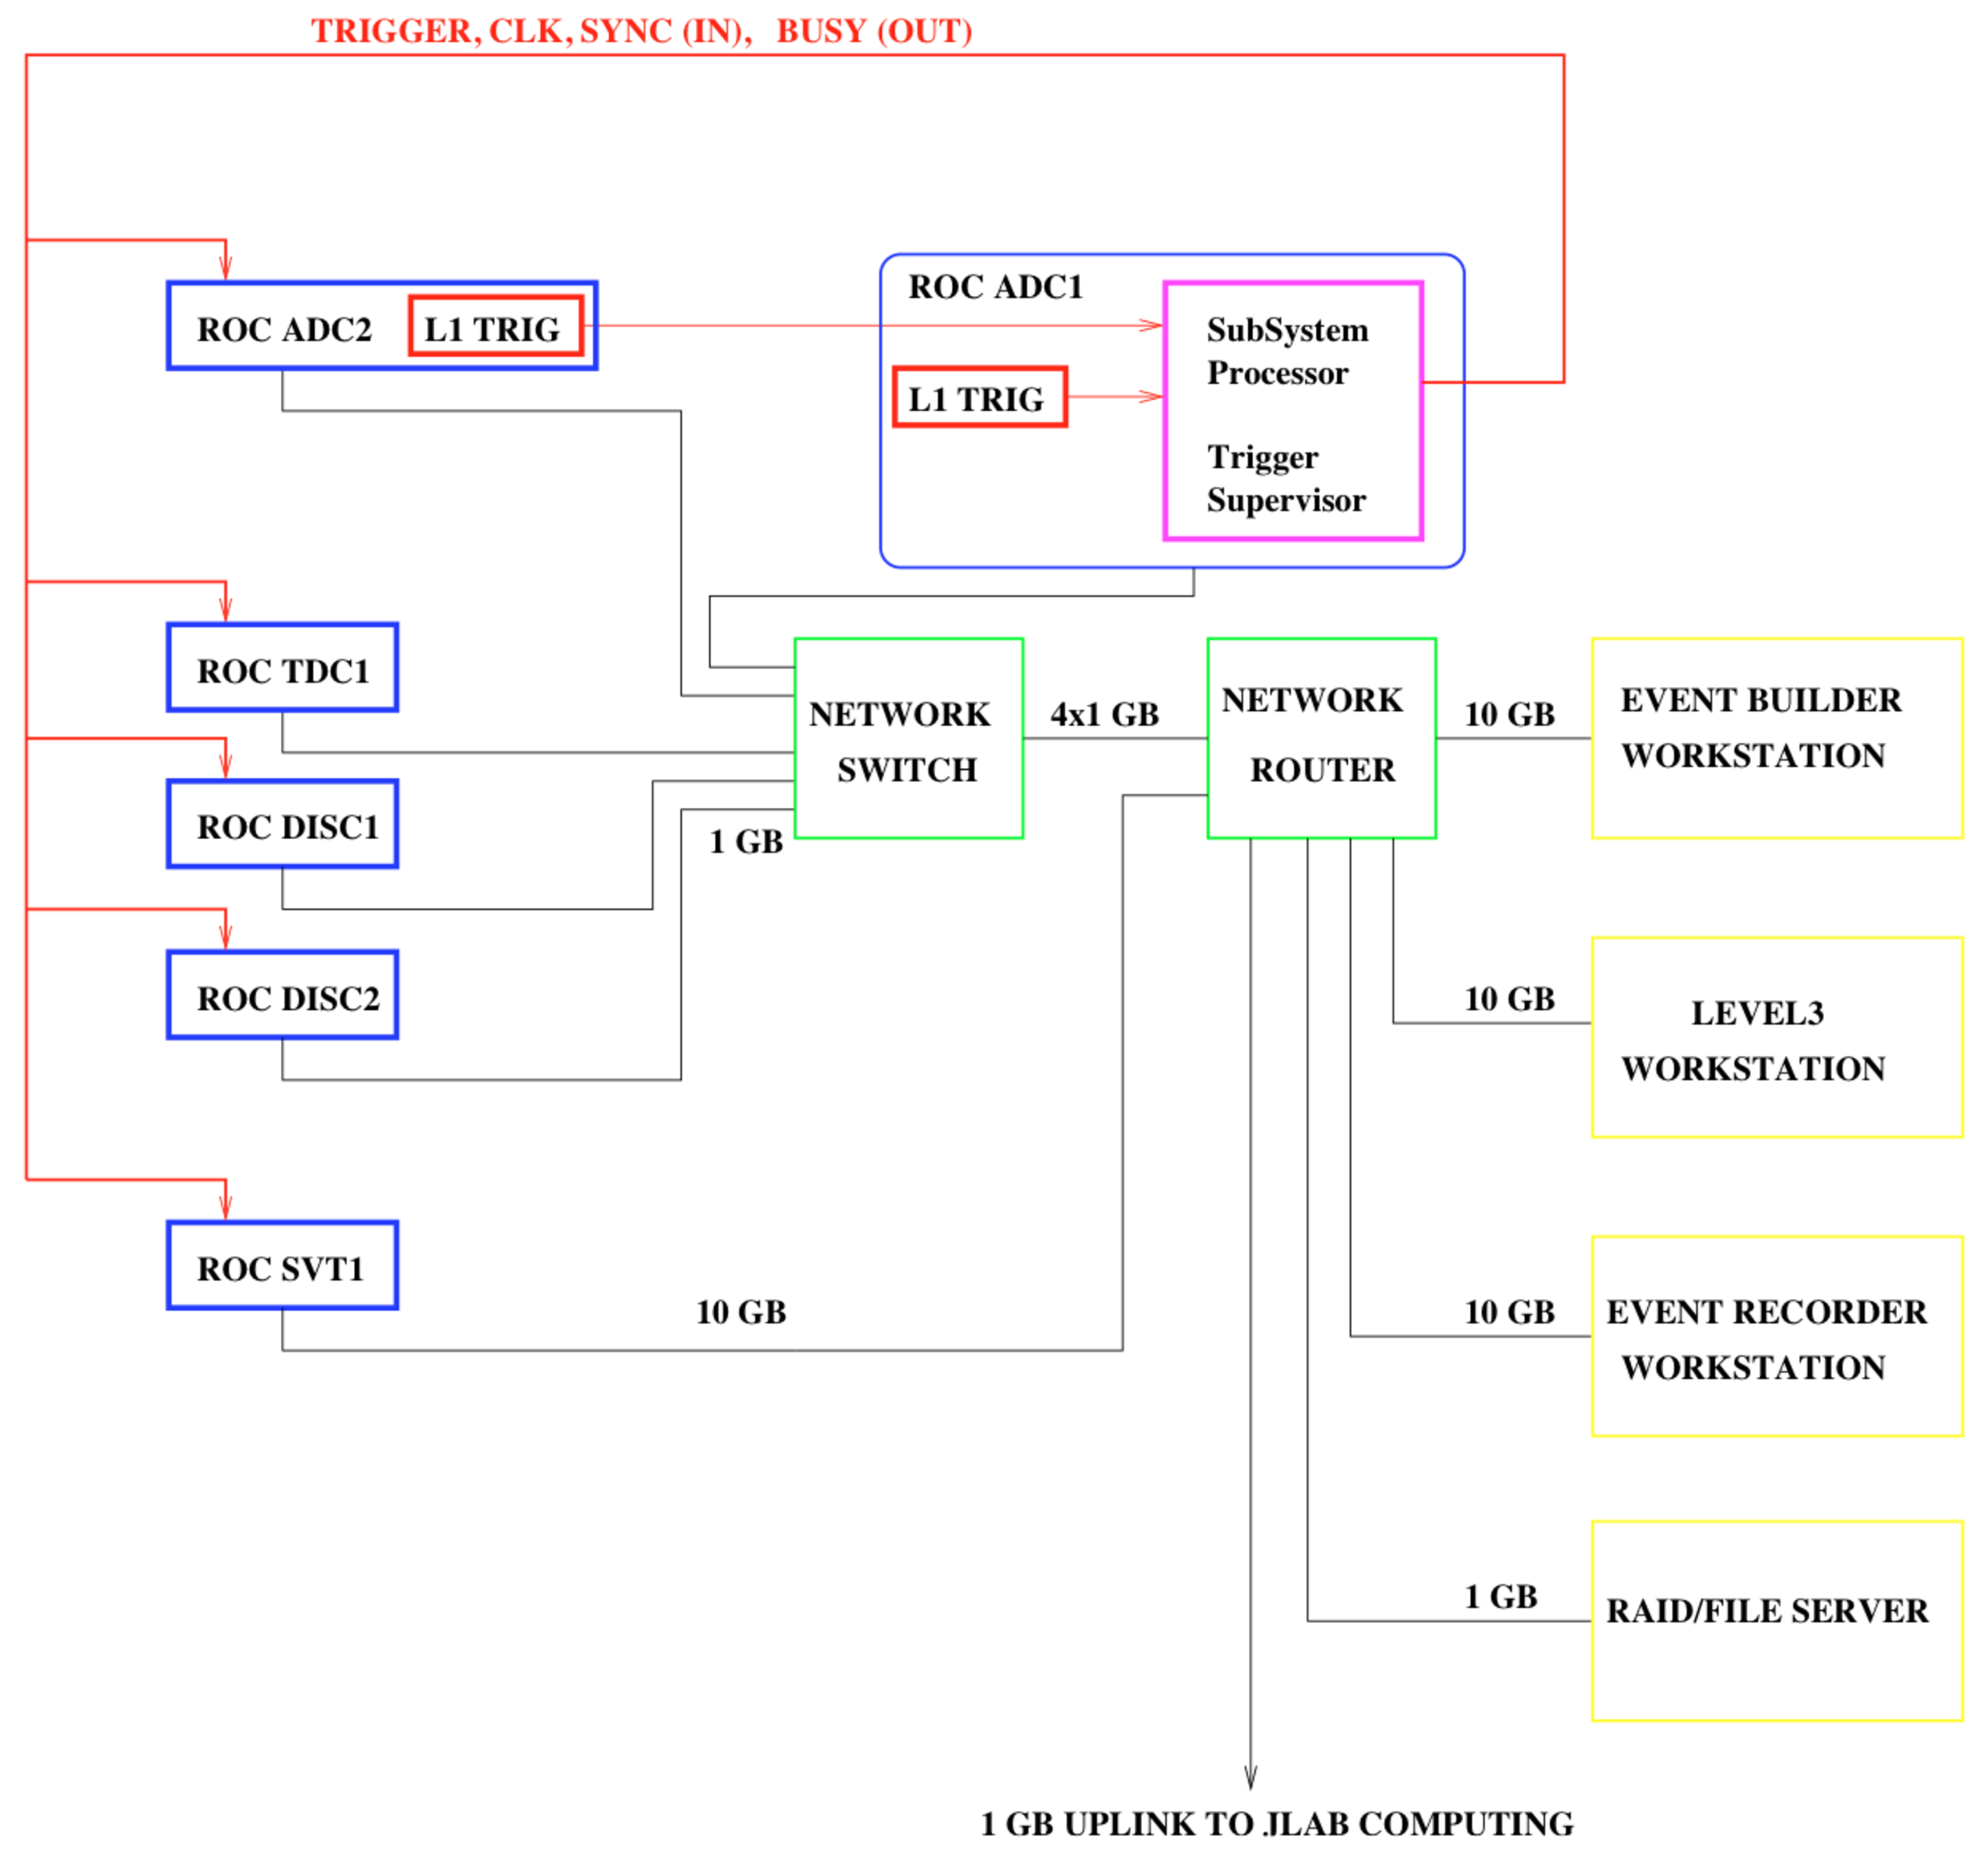
\includegraphics[scale=0.35]{test2012/daq/daq_schem.pdf}
\caption{\small{Readout and processing system block diagram.}}\label{fig:daq}
\end{figure*}
The front-end systems of the ECal and SVT are similar. 
The differences of the DAQ and trigger w.r.t. to the HPS are fleshed out in greater detail below but 
are all related to the following areas:
\begin{enumerate}
\item a lower ECal cluster resolution and no calibration available at the trigger level together with simpler trigger logic, 
\item a smaller SVT without the need for optical readout and power distribution inside the vacuum,
and
\item lower bandwidth links.
\end{enumerate}

The two front-end electronics systems for the ECal and SVT are essentially unchanged. The ECal provides 
input to the Level~1 trigger system after which an accepted event is acquired from the two sub-systems 
and are processed in the data acquisition and processing system. The Readout Crate Controllers (ROCs)
 described for HPS are unchanged and installed in every VME, VME64X, VXS crates running 
 mvme6100 controllers with a prpmc880 or pmc280 co-processor modules. A hybrid approach was 
 used for the SVT DAQ in the test run where the ROC ran on a external PC connected to the ATCA crate. 
 Similar to HPS, a Foundry Router was used as the backbone of the DAQ system, providing 1Gbps and 
 10Gbps connections between components and to the JLAB Computer Center.

The Event Builder, Event Recorder, and other critical DAQ components ran on 
4-CPU Opteron-based servers, which was sufficient for the test run. The RAID5 test run storage system 
had a 100~MByte/sec capability which was well enough for the data rates attained in the test run as 
described below. 

%\subsubsection{SVT DAQ}



The SVT DAQ is a SLAC built data acquisition system utilizing the Advanced Telecommunication Computing Architecture (ATCA) for high speed data transfer.  It is designed to readout data continuously at 40 MHz from the silicon detector modules, and transfer data to the JLab DAQ once a trigger signal is received. It can support a trigger rate of a few 10�s of kHz.

There are a total of 20 silicon strip sensors, each one connected to an onboard readout card called a hybrid which holds five 128-channel APV25 integrated circuits. The APV25s provide amplification, pipelining, and analog storage for trigger accepted events. There are 5 analog outputs for each 640-channel hybrid. Each hybrid will be connected via a multi-twisted-pair cable to a readout board.

 \begin{figure}[t]
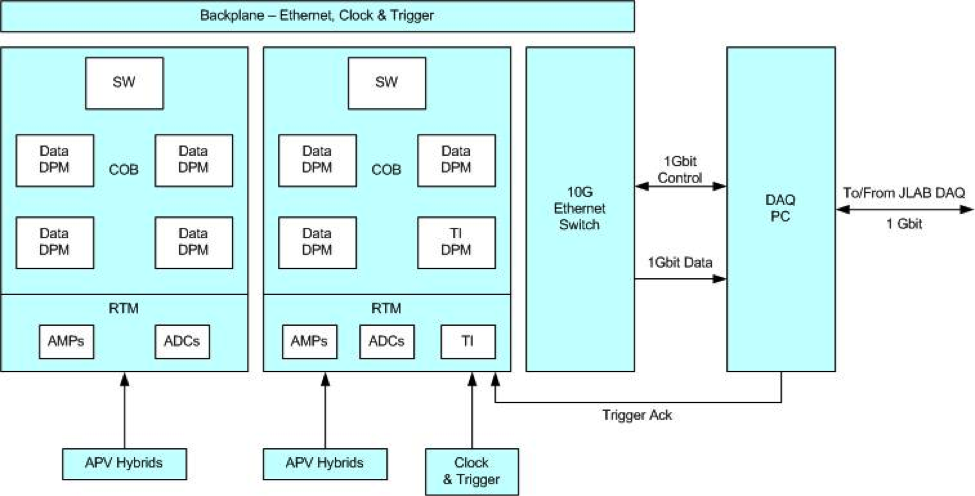
\includegraphics[scale=0.9]{test2012/daq/svt_daq_diagram.png}
\caption{\small{Schematic of the SVT DAQ showing input from the hybrids mounted on the silicon detector to the RTM, its connection to the COB, and the Ethernet switch used to transfer data a 1 Gbit/sec to the DAQ PC and ultimately to the JLAB DAQ. Details are given below.}}\label{fig:svtdaq}
\end{figure}


The SVT readout system is shown in Figure \ref{fig:svtdaq}. The outputs of 12 hybrids are digitized on an ATCA (Advanced Telecommunication Computing
Architecture) RTM (Rear Transition Module) board. A pre-amplifier converts the APV25 differential current output to a different voltage output scaled to the sensitive range of a 14-bit ADC. The RTM is organized into 4 sections with each section supporting 3 hybrids (15 channels). The ADC is operated at the system clock of 41.667 Mhz. The RTM also includes a 4-channel Fiber Optic module and supporting logic which can be used to interface to the JLAB trigger supervisor card.

On the ATCA main board (also known as the Cluster On Board or COB), shown in Figure \ref{fig:svtdaqmodule}, there are 4 FPGAs each interfacing to a single section of the RTM. Each FPGA exists on a separate daughter card known as the Data Processing Module or DPM. The DPMs receive the digitized data from the RTM ADCs, apply thresholds for data reduction and organize the sample data into UDP datagrams. The DPMs also host an I2C controller used to configure and monitor the APV25 chips. One DPM in the system is configured to operate as a trigger interface module, receiving and distributing the system clock and trigger to the rest of the ATCA crate.
The ATCA crate hosts 2 COB cards, one supporting 4 data processing DPMs and the other supporting 3 data processing DPMs and one trigger DPM. A total of 21 hybrids are supported, 1 more than the 20 required. The two ATCA COB cards and their DPMS are interconnected with a 10G switch card which also hosts two external 1Gbit Ethernet interfaces to a standard PC.

 \begin{figure}[t]
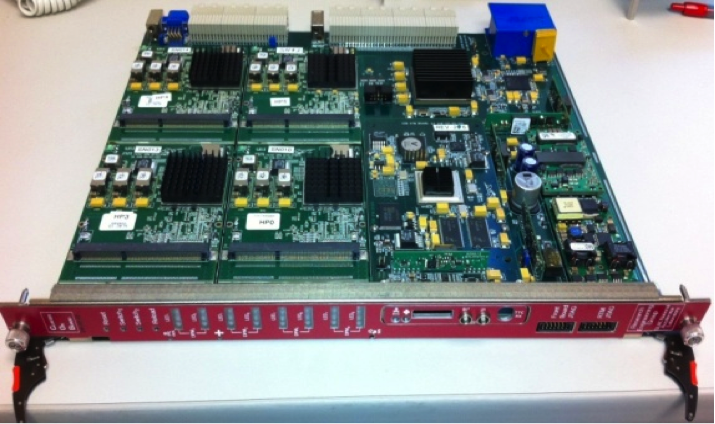
\includegraphics[scale=0.9]{test2012/daq/svt_daq_module.png}
\caption{\small{The Cluster on Board (COB) board, the main board of the SVT DAQ. The RTM is plugged into the COB in the back.}}\label{fig:svtdaqmodule}
\end{figure}


The external PC supports three network interfaces, 2 standard 1G-bit Ethernet and one custom low latency data reception card. The first Ethernet interface is used for slow control and monitoring of the 8 DPM modules. The second Ethernet interface serves as the interface to the JLAB data acquisition system. The third custom low latency network interface is used to receive data from the SVT ATCA crate and supports a low latency, reliable TTL trigger acknowledge interface to the trigger DPM. This PC hosts the SVT control and monitoring software as well as the JLAB ROC (Read Out Controller) application.



Signals from each module are sent to a signal splitter. One of the outputs of the splitter is fed to a discriminator that also has an internal scaler, and then to a TDC channel. The other output is sent to the Jefferson Lab FADC250 VXS module, Figure \ref{fig:fadc}. Two FADC crates are required for the  two modules. The trigger from the ECal is based on FADC information and includes a cluster finding algorithm using FPGA modules. It is described in Section \ref{trigger}. With the FADCs, the energy of clusters will be determined at the crate trigger level and will be used in making the trigger decision.

\begin{figure}[t]
\includegraphics[scale=0.5]{test2012/daq/FADC250_Photo_001.jpg}
\caption{\small{FADC250 VXS module.}}\label{fig:fadc}
\end{figure}




